\documentclass[a4paper]{article}
\usepackage{latexsym}
\usepackage[a4paper]{geometry}
\usepackage{color}
\usepackage{listings}
\usepackage[pdftex]{graphicx}
\usepackage{float}

\definecolor{Blue}{rgb}{0,0,0.5}
\definecolor{Green}{rgb}{0,0.75,0.0}
\definecolor{LightGray}{rgb}{0.6,0.6,0.6}
\definecolor{DarkGray}{rgb}{0.3,0.3,0.3}
\lstset{language=Matlab,
   keywords={function,uint8,uint16,uint32,double,break,case,catch,continue,else,elseif,end,for,global,if,otherwise,persistent,return,switch,try,while},
   basicstyle=\ttfamily\small,
   breaklines=true,
   keywordstyle=\bfseries\color{Blue},
   commentstyle=\itshape\color{LightGray},
   stringstyle=\color{Green},
   numbers=left,
   numberstyle=\tiny\color{DarkGray},
   stepnumber=1,
   numbersep=10pt,
   backgroundcolor=\color{white},
   tabsize=2,
   showspaces=false,
   showstringspaces=false,
   captionpos=b}

%Boldface text for type writer font
\usepackage{bold-extra} %\DeclareFontShape{OT1}{cmtt}{bx}{n}{<5><6><7><8><9><10><10.95><12><14.4><17.28><20.74><24.88>cmttb10}{}

%Break words properly at the end of a line (which isn't sloppy...)
\sloppy

%Use command \exercise for each exercise
\newcounter{exerciseCount}
\setcounter{exerciseCount}{0}
\newcommand{\exercise}[1]{\addtocounter{exerciseCount}{1} \noindent \medskip {\large \textsf{\textbf{Exercise \arabic{exerciseCount} \--- #1}}} \par}
\renewcommand{\theenumi}{\textsf{\textbf{\alph{enumi}}}}

%Use command \code for code snippets
\newcommand{\code}[1]{\textnormal{\texttt{#1}}}

\title{\textsf{Image Processing \\ lab 5}}
\author{Klaas Kliffen \and Jan Kramer}
\date{\today}

\begin{document}
\maketitle

\exercise{Edge detection}
\begin{enumerate}
\item
\lstinputlisting{../lab5ex1/IPMarrHilderth.m}
\item
\begin{figure}[H]
\centering
\begin{tabular}{cc}
    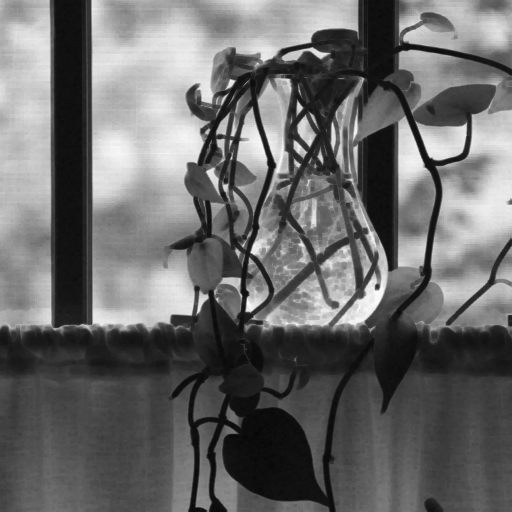
\includegraphics[width=0.3\textwidth]{../lab4ex2/gerode.png} & 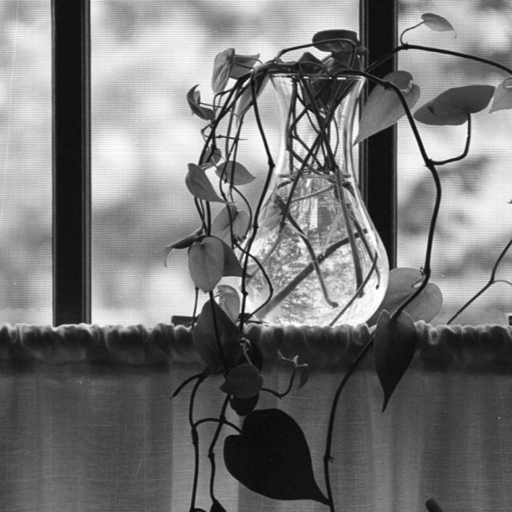
\includegraphics[width=0.3\textwidth]{../lab4ex2/vase.png} \\
    The erosion & Original image & The dilation \\
\end{tabular}
\caption{TODO}
\label{fig:marrhil}
\end{figure}
\end{enumerate}


\exercise{Region splitting and merging}
\begin{enumerate}
\item
\item
\lstinputlisting{../lab5ex2/IPpredicate.m}

\end{enumerate}

\exercise{Fourier descriptors}
\begin{enumerate}
\item
\lstinputlisting{../lab5ex3/IPcontour.m}
\item
\item
\lstinputlisting{../lab5ex3/IPfourierdescr.m}
\item
\end{enumerate}

\newpage
\section*{Task distribution}

\begin{table}[H]
\centering
\begin{tabular}{ccccc}
ex1 & design & implementation & answers questions & writing report \\
\hline
Klaas & 20\% & 10\% & 20\% & 40\% \\
\hline
Jan & 80\% & 90\% & 80\% & 60\% \\
\end{tabular}
\end{table}

\begin{table}[H]
\centering
\begin{tabular}{ccccc}
ex2 & design & implementation & answers questions & writing report \\
\hline
Klaas & 50\% & 20\% & 25\% & 25\% \\
\hline
Jan & 50\% & 80\% & 75\% & 75\% \\
\end{tabular}
\end{table}

\begin{table}[H]
\centering
\begin{tabular}{ccccc}
ex3 & design & implementation & answers questions & writing report \\
\hline
Klaas & 80\% & 75\% & 75\% & 80\% \\
\hline
Jan & 20\% & 25\% & 25\% & 20\% \\
\end{tabular}
\end{table}

\end{document}
